\documentclass[../CSC_5RO17_TA_TP1.tex]{subfiles}

\begin{document}
\subsection{Question 1}
\noindent Une \textbf{homographie} est une transformation projective entre deux plans $\pi_1$ et $\pi_2$ qui conserve les droites. Une \textbf{homographie} peut être représentée par l'équation suivante:
\begin{equation}
    \boxed{
        \underbrace{
            \begin{bmatrix}
            x_2\\ y_2\\ 1
            \end{bmatrix}
        }_{\mathbf{x}_{\pi_{2}}\in\pi_2}
        =
        \underbrace{
            \begin{bmatrix}
                a_{11} & a_{12} & t_x\\
                a_{21} & a_{22} & t_y\\
                v_1    & v_2    & 1\\
            \end{bmatrix}
        }_{\mathbf{H}\text{, Homographie}}
        \times
        \underbrace{
            \begin{bmatrix}
                x_1\\ y_1\\ 1
            \end{bmatrix}
        }_{\mathbf{x}_{\pi_{1}}\in\pi_1}
    }
\end{equation}
Où:
\begin{enumerate}[noitemsep, rightmargin=\leftmargin]
    \item \textbf{Vecteur de translation} : responsable de la translation de l'image selon les axes $x$ et $y$.
    \begin{equation}
        \mathbf{t} = \begin{pmatrix}t_x & t_y\end{pmatrix}^\intercal
    \end{equation}
    \item \textbf{Vecteur de relation} : responsable de la distorsion des relations entre les points et les droites à l'infini.
    \begin{equation}
        \mathbf{v} = \begin{pmatrix}v_1 & v_2\end{pmatrix}
    \end{equation}
    \item \textbf{Matrice d'affinité} : responsable du changement de l'image tout en préservant les droites parallèles et les aires.
    \begin{equation}
        \mathbf{A}_f = \begin{bmatrix} a_{11} & a_{12}\\ a_{21} & a_{22}\end{bmatrix}
    \end{equation}
\end{enumerate}
\noindent En termes simples, cela signifie que si deux images d'une scène sont prises sous certaines conditions géométriques, la relation entre ces images peut être modélisée par une \textbf{homographie}. Cas où la transformation est une homographie:
\begin{enumerate}[noitemsep, rightmargin=\leftmargin]
    \item images d'un même plan vues sous deux poses 3D différentes;
    % \begin{figure}[H]
    %     \centering
    %     \includegraphics[width=135mm, page=25]{../CSC_5RO17_TA cours_homographie.pdf}
    %     \caption{Différent 3D poses}
    %     \label{fig_2_3d_positions}
    % \end{figure}
    \item images prises par une caméra tournant autour de son centre optique;
    % \begin{figure}[H]
    %     \centering
    %     \includegraphics[width=135mm, page=24]{../CSC_5RO17_TA cours_homographie.pdf}
    %     \caption{Rotation centre optique}
    %     \label{fig_rotation_optical_center}
    % \end{figure}
\end{enumerate}
\end{document}
